\begin{frame}
    \frametitle{El Teorema de CAP}

    \begin{columns}
        \column{.6\textwidth}
        \centering
        \includegraphics<2-10>[height=\textheight]{distributed-db.jpg}

        \column{.4\textwidth}
        \centering

        \only<3->{
            \only<7->{{\Large Elige 2:}}
        \begin{itemize}
            \item \red<4,8,9>{Consistencia} \only<3>{(\textit{\red{C}onsistency})}
            \item \red<5,8,10>{Disponibilidad} \only<3>{(\textit{\red{A}vailability})}
            \item \red<6,9,10>{Tolerancia a particiones} \only<3>{(\textit{\red{P}artition tolerance})}
        \end{itemize}

        }
        \only<7>{
        \begin{flushright}
            \small
            \textit{por Eric Brewer, 2000;}

            \textit{demostrado por Seth Gilbert y Nancy Lynch, 2002.}
        \end{flushright}
        }
    \end{columns}

\end{frame}

\begin{frame}
    \frametitle{El Teorema de CAP}

    \centering
    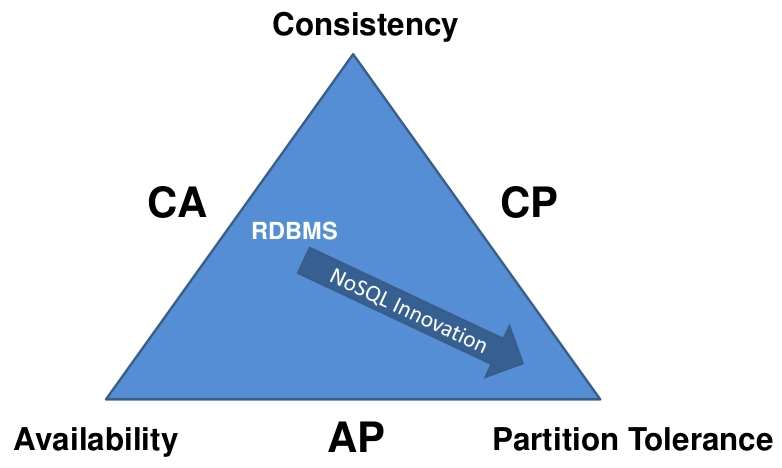
\includegraphics[scale=.7]{cap-theorem.jpg}

\end{frame}